\subsubsection{\stid{1.13} SOLLVE} \label{subsubsect:sollve}


\paragraph{Overview} 

OpenMP is a   directive-based API for shared-memory and accelerator systems. It
is supported by a stable community of vendors, research labs, and academics who
participate in the efforts of the  OpenMP Architecture Review Board; it is
one of the most used API for intra-node programming in ECP applications.
Implementations are available in all DOE LCFs, and a variety of programming
tools are available to support OpenMP application development. The mission of
the SOLLVE project is to further enhance the OpenMP specification and
implementations to meet the performance and productivity goals of ECP
applications. We directly interact with DOE end-users in order to understand
their application software requirements. We will develop OpenMP solutions for
ECP needs; propose features for standardization; produce prototype
implementations of new features to support their rapid adoption; develop and
deliver a verification and validation (V\&V) suite to assess implementations and
enable evaluations by DOE  facilities, and deliver a high-quality,  robust ECP
OpenMP implementation in the LLVM compiler framework. Attaining high levels of
single-node performance and meeting performance portability needs will only be
possible via enhancements to OpenMP in such areas as memory management (e.g. allocators) for 
complex memory  hierarchies, data motion to/from accelerators, descriptive / prescriptive
loop constructs and meta directives that allow the creation of performance portable code. 
SOLLVE plays a critical
role in identifying, implementing, promoting, and deploying key functionality
that will enable ECP application developers to reach their goals using OpenMP.
We will demonstrate the high impact of new features via their use in selected
ECP applications.

\paragraph{Key  Challenges}
%\textit{Describe what is hard to do, why it is challenging.}
The SOLLVE project addresses a number of key challenges faced by DOE facilities,
application groups and scientists. The first of these is the gap between
existing OpenMP functionality and user requirements. This problem is largely
exacerbated by ever increasing complexity and heterogeneity of computing
systems.
The second challenge is to suitably evolve the OpenMP specification to satisfy
the identified requirements. This process involves coordinating with vendors
and other members of OpenMP's language committee  to reach consensus on the scope of the API, syntax and semantics of new features.
The third challenge addressed by the SOLLVE project is performance portability.
Current hardware and software trends 
\cite{exascale-roadmap.ijhpca.2011}
 have shown that
pre-Exascale and Exascale systems will be extremely heterogeneous, and may 
consist of  diverse architectures such as
CPUs, GPUs, FPGAs, among others. Programmatically, this means %adaptively 
there will be a need to orchestrate  
work and data on multiple types of memories with local computational units, accelerators, while exposing several distinct kinds of 
 parallelism (e.g. tasks, worksharing, SIMD) 
to achieve suitable performance levels on different architectures.
This naturally places heavy emphasis on application readiness, where APIs such as 
OpenMP will need to address 
performance portability to serve the critical role
of abstracting hardware and software complexities.
Finally, the last challenge is to fully assess the quality of delivered
OpenMP implementations, their compliance with the specification and potential
divergence that, if unidentified, could can lead to undesired program behavior.
% and, ultimately, errors
%that can consume significant amount of resources to repair.


\paragraph{Solution Strategy}
The challenges discussed here are addressed by the SOLLVE project's five major thrust areas, which
we describe below:
% as part of the SOLLVE process:
%rewrite??
%\textit{Describe your basic strategy for addressing the challenges.}

\begin{enumerate}
\item {\bf Application requirements}
The first step of the SOLLVE process consists of collecting user requirements
from relevant and representative ECP applications (e.g. QMCPACK or Lattice QCD).
The resulting requirements are then converted to use cases which are shared with
 the OpenMP Architecture Review Board's Language Committee.
\item {\bf OpenMP specification evolution}
This thrust area is responsible for designing new (or adapting existing) OpenMP features to 
meet the needs identified in the use cases and proposing them to the OpenMP committee. 
%of translating use-cases to new OpenMP
%features to be introduced into the standard. 
 %In this phase, the 
  The semantics
of the new capabilities are defined and formalized, followed by early
prototypes in one or more OpenMP implementations (either vendor or open
source solutions).  %The bulk of 
Most new features fall into the areas
of accelerator support, affinity, tasking or memory management.
\item {\bf Lightweight OpenMP runtime}
SOLLVE is committed to deliver an open source, lightweight and scalable
OpenMP implementation (the BOLT runtime) that will fulfill ECP needs.
This thrust serves two key objectives: i) early access to a stable 
implementation; and ii) risk mitigation.
\item {\bf LLVM }
This compiler infrastructure is ideal for 
delivering high-quality and deployable OpenMP implementations.
Our effort enhances the LLVM framework by introducing compiler transformations
that leverage both prototyped OpenMP features and those introduced
in the latest specifications.  % (4.5, 5.0). 
User adoption of new OpenMP capabilities can vary from
months to years. Thus, delivering compiler technology that automatically translates 
user code including new OpenMP functionality (e.g. target offloading with
data mappers), represents high return value for ECP in terms of time and
resources. 
\item {\bf Validation and verification (V\&V)} This thrust focuses on
designing and implementing a benchmark suite that makes it possible to assess the coverage
and standard compliance of several OpenMP implementations (LLVM, BOLT, IBM XL,
NVIDIA, etc). In addition, a ticket system for bug reporting and inquiries has
 been deployed to facilitate interaction with end users.
\end{enumerate}

\paragraph{Recent Progress}
%Figure \ref{fig:sollve-update} shows the latest progress on the five core SOLLVE
%thrust areas. We note that the {\bf training and outreach} activity is a
%cross-cutting effort which includes resources from the SOLLVE project and
%external partners, namely collaborators from Lawrence Berkeley National
%Laboratory, Oak Ridge, University of Delaware and other academic institutions.
%In addition to the above updates, a number of articles have also been published
%as part of the SOLLVE effort \cite{openmp-tr6,zinenko.cc.2018,osti_1429981,DBLP:conf/sc/MishraLKFC17}.
Figure \ref{fig:sollve-update} shows the latest progress on the five core SOLLVE thrust areas. 
%We note that the training and outreach activity is a cross-cutting effort which
%includes resources from the SOLLVE project and external partners, namely
%collaborators from Lawrence Berkeley National Laboratory, University of
%Delaware, vendors such as Intel and NVidia, and other institutions.
In preparation for the OpenMP 5.0 release, we organized a number of OpenMP-oriented hackathons 
\cite{bnl.knl-hackathon.2018,bnl.gpu-hackathon.2018}, webinars,
and tutorials 
%in the ECP Annual Meeting, the Super Computing Conference (SC)
%and the International Conference on Supercomputing (ICS)
\cite{sollve.ecp-am.tutorial.2018,sollve.ecp.webinar.2018,sollve.ecp-am.tutorial.2019,openmp.sc.tutorial.2018a,openmp.sc.tutorial.2018b}.
%In addition to the above updates th, a number of articles have also been published
%as part of the SOLLVE effort [2, 3, 4, 5].
%In addition to delivering an enhanced OpenMP specification and implementation,
%the team members and collaborators of the SOLLVE ECP project have also produced
%several high-quality articles published in both peer-reviewed venues and open
%access repositories. 
The SOLLVE effort has also produced several articles,
including the major milestones leading to the OpenMP 5.0 specification
\cite{openmp-tr6,openmp.spec.5.0}, 
synergistic compiler and run-time optimizations
\cite{zinenko.cc.2018,DBLP:conf/sc/MishraLKFC17,li.iwomp.2018,bertolacci.iwomp.2018,scogland.iwomp.2017,kruse.arxiv.2018b,kruse.arxiv.2018a,doerfert.iwomp.2018,kong.arxiv.2018},
evaluation of OpenMP implementations 
\cite{osti_1429981,openmpevol.2018, diaz.iwomp.2018,diaz.icpp.2018},
and several run-time extensions for flexible and efficient execution
\cite{seo2018,kemp.iwomp.2018,bolt.git,iwasaki2018}.

\begin{figure}[t]
\centering
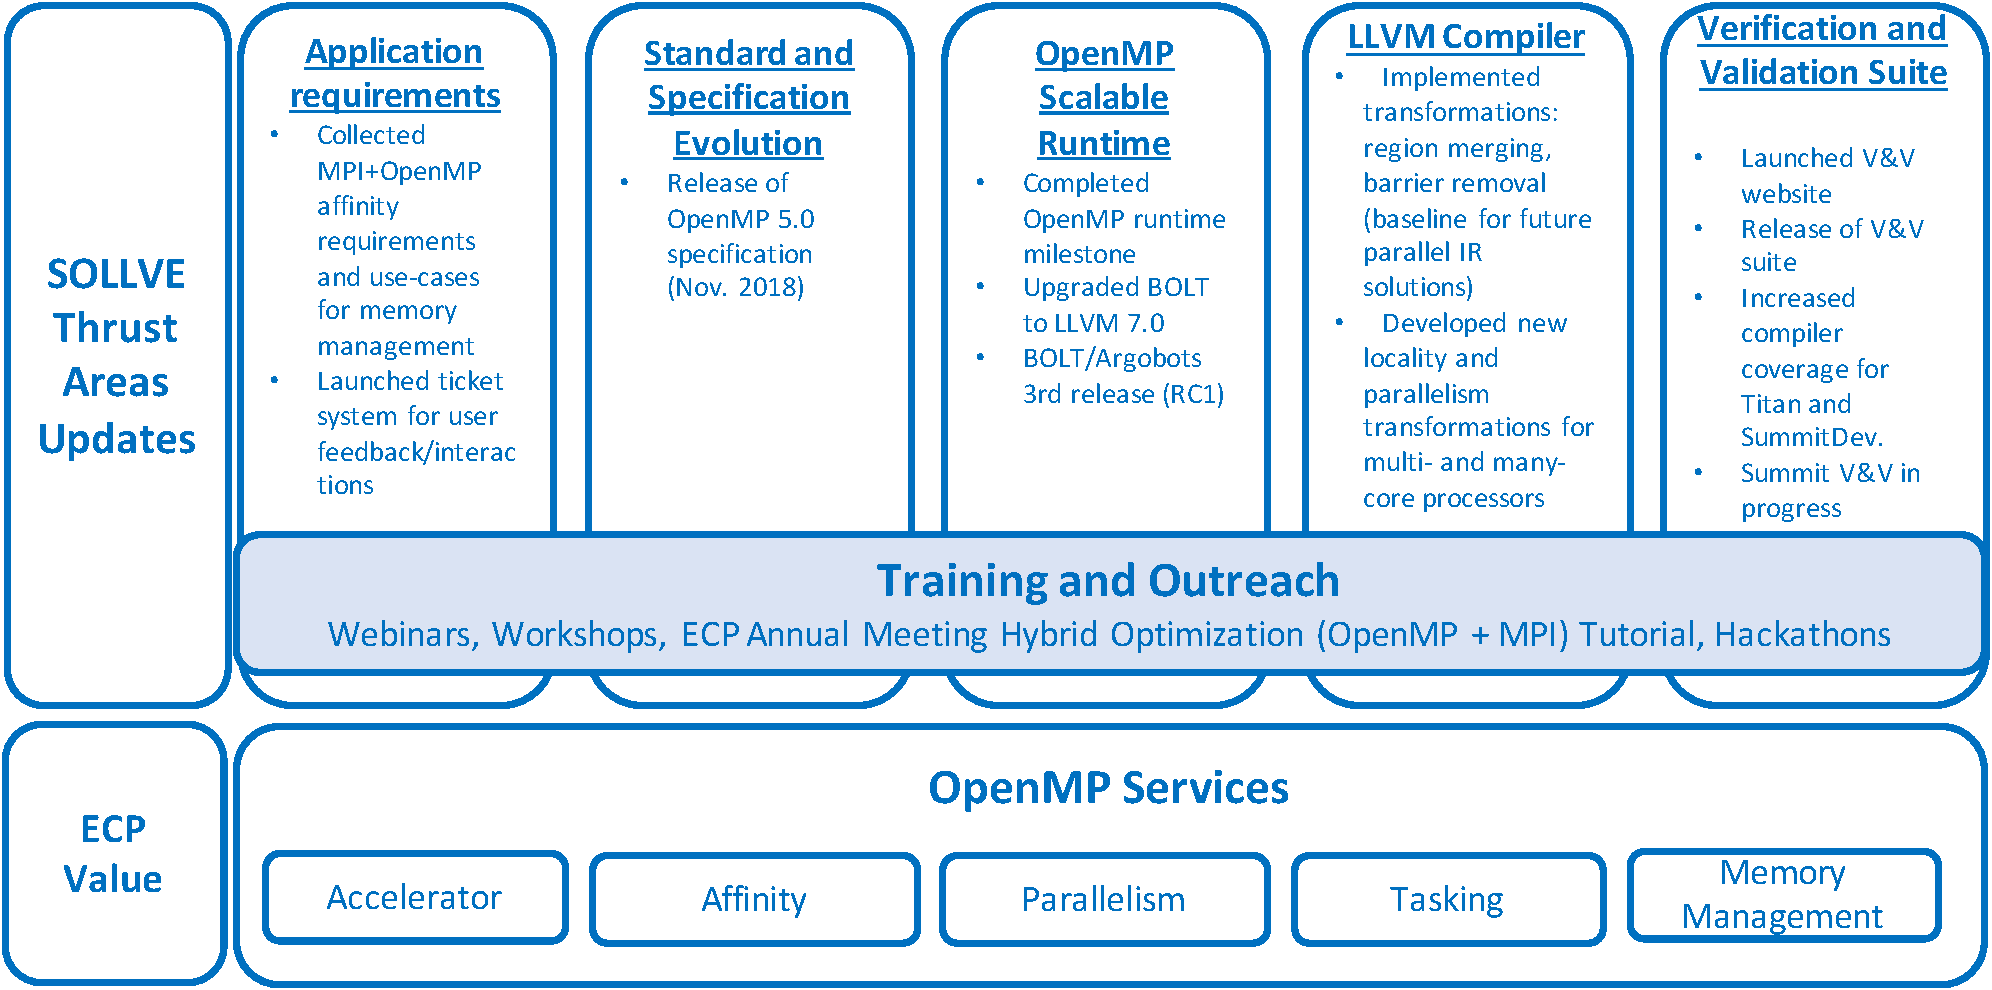
\includegraphics[width=0.9\linewidth]{projects/2.3.1-PMR/2.3.1.13-SOLLVE/SOLLVE-progress}
\caption{\label{fig:sollve-update}SOLLVE thrust area updates}
\end{figure}

\paragraph*{Next Steps}
 The next steps planned for SOLLVE are:
\begin{itemize}
\item Applications: gather more requirements for  the new memory management API and loop construct; prepare and coordinate OpenMP webinars focusing on 
the new features available in OpenMP 5.0.
Develop and deliver hackathons. 
\item OpenMP standard: Participate in upcoming face-to-face meetings; % (next is in January); 
 prioritize features for OpenMP 5.1 (e.g. exposing streams to OpenMP, new APIs for multiple devices, etc).
\item OpenMP runtime: tighter integration with the other SOLLVE components and hardening the BOLT stack with more applications and validation suites.
\item LLVM compiler: develop new optimizations leveraging prototype parallel-IR; refine Clang based implementation of data layout transformations; evaluate new compiler transformations on ECP testbeds.
\item V\&V suite: identify performance critical kernels from selected applications; prepare for next releases;  %(e.g. ; 
 coordinate suite deployment with CORAL systems.
\end{itemize}

